\chapter{Boolean Logic}
\chaplabel{logic}

\section{Introduction}
This chapter introduces some basic Boolean logic including gates and Boolean algebra.

When can you drive through an intersection? When the light is NOT red. This is the first and simplest
logic operator--the NOT element. It simply changes any TRUE to FALSE or FALSE to TRUE (you can substitute
1 for TRUE and 0 for FALSE, or on/off).

How do you start a car? In most of the cars I have driven I have to press on the brake at the 
same time as I turn the key. To say it another way, the car starts when I press the break
AND turn the key.
\begin{equation}
	pressBreak \: \mathrm{AND} \: turnKey = startedCar
\end{equation}
Again on a car, a particular blinker light will turn on if you turn on the turn signal or if you turn on the 4-way blinker.
\begin{equation}
	turnSignal \: \mathrm{OR} \: 4wayBlinker = blinking
\end{equation}
The AND and OR in the equation are Boolean operators. 

\section{Methods of Representing Logic}
It is important to differentiate between different forms of representation because $\overline{\mathrm{EN}}$
means \textbf{active low} enable. It does not mean NOT(E AND N). The understanding of which method is being 
used is usually derived from context. Using the dot ($\cdot$) everywhere can become burdensome, so when context
makes it obvious (usually examples involving A, B, and C or X and Y) we may drop the dots and just use adjacency to represent
the AND function.

\section{Boolean Algebra}

\subsection{Theorems of Boolean Algebra}
Ways to show NOT:
\begin{subequations}
	\begin{align}
	NOT(X) &= \overline{X} = X^{\prime} \\
	\overline{(\overline{X})} &= \left(X^{\prime}\right)^{\prime}= X
	\end{align}
\end{subequations}
Rules of AND and OR:
\begin{subequations}
	\begin{align}
	\mathrm{AND} \qquad & \mathrm{OR}\notag\\
	0\cdot0 = 0 \qquad & 1+1 = 1\\
	1\cdot1 = 1 \qquad & 0+0 = 0\\
	0\cdot1 = 1\cdot0 = 0 \qquad & 1 + 0 = 0 + 1 = 1
	\end{align}
\end{subequations}

\begin{subequations}
	\begin{align}
	\mathrm{AND} \qquad & \mathrm{OR}\notag\\
	X\cdot1 = X \qquad & X + 0 = X\\	
	X\cdot0 = 0 \qquad & X + 1 = 1\\	
	X\cdot X = X \qquad & X + X = X\\	
	X\cdot\overline{X} = 0 \qquad & X + \overline{X} = 1
	\end{align}
\end{subequations}

For two and three variables you have the following useful equations:
\begin{subequations}
	\begin{align}
	\mathrm{AND} \qquad & \mathrm{OR}\notag \\
	X\cdot Y = Y \cdot X \qquad & X + Y = Y + X \\
	(X \cdot Y) \cdot Z = X \cdot (Y \cdot Z) \qquad & (X + Y) + Z = X + (Y + Z) \\
	(X + Y)\cdot (X + Z) = X + Y\cdot Z \qquad & X\cdot Y + X\cdot Z = X\cdot (Y + Z) \\
	X\cdot (X + Y) = X \qquad & X + X\cdot Y = X \\
	(X + Y) \cdot (X + \overline{Y}) = X \qquad & X\cdot Y + X\cdot \overline{Y} = X \\
	X\cdot (\overline{X} + Y) = X\cdot Y \qquad & X + \overline{X} \cdot Y = X + Y
	\end{align}
	\begin{equation}
	X\cdot Y + \overline{X}\cdot Z + Y\cdot Z = X\cdot Y + \overline{X}\cdot Z \\
	\end{equation}
	\begin{equation}
	(X + Y) \cdot (\overline{X} + Z) \cdot (Y + Z) = (X + Y) \cdot (\overline{X} + Z)
	\end{equation}
\end{subequations}

A very important pair of equations are DeMorgan's theorems which allow us to switch between sums of 
products and products of sums.
\begin{subequations}
	\begin{align}
		\overline{(X_1\cdot X_2 \cdot \ \cdots\  \cdot X_n)} & = \overline{X_1} + \overline{X_2} + \cdots + \overline{X_n} \\
		\overline{(X_1 + X_2 + \cdots + X_n)} & = \overline{X_1}\cdot\overline{X_2}\cdot\ \cdots\ \cdot\overline{X_n}
	\end{align}
\end{subequations}

The following are very important to remember:
\begin{subequations}
	\begin{align}
		\overline{A} \cdot \overline{B} &\neq \overline{AB} \\
		\overline{A} + \overline{B} &\neq \overline{A + B} 
	\end{align}
\end{subequations}

\section{Logic Gates and Truth Tables}
It is important to be able to transform between equation, diagrams/circuits, and truth tables.
\begin{figure}[!htb]
	\centering
	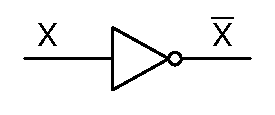
\includegraphics[scale=0.7]{logic/NOT.eps}
	\caption{The NOT gate, also called an inverter, outputs NOT(A).}
	\label{fig:notgate}
\end{figure} 

\begin{table}[!ht]
	\centering
	\begin{tabular}{| c | c |}
		\hline
		A & X \\ 
		\hline
		0 & 1 \\ \hline
		1 & 0 \\ \hline
	\end{tabular}
	\caption{This is the truth table for a NOT gate.}
	\label{table:notgate}
\end{table}

\begin{figure}[!htb]
	\centering
	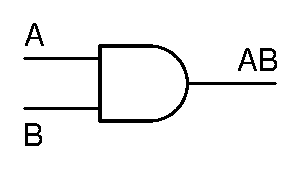
\includegraphics[scale=0.7]{logic/AND.eps}
	\caption{The AND gate outputs A AND B.}
	\label{fig:andgate}
\end{figure} 

\begin{table}[!ht]
	\centering
	\begin{tabular}{| c | c | c |}
		\hline
		A & B & X \\ 
		\hline
		0 & 0 & 0 \\ \hline
		0 & 1 & 0 \\ \hline
		1 & 0 & 0 \\ \hline
		1 & 1 & 1 \\ \hline
	\end{tabular}
	\caption{This is the truth table for an AND gate.}
	\label{table:andgate}
\end{table}

\begin{figure}[!htb]
	\centering
	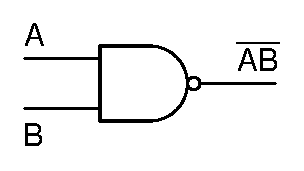
\includegraphics[scale=0.7]{logic/NAND.eps}
	\caption{The NAND gate outputs NOT(A AND B).}
	\label{fig:nandgate}
\end{figure} 

\begin{table}[!ht]
	\centering
	\begin{tabular}{| c | c | c |}
		\hline
		A & B & X \\ 
		\hline
		0 & 0 & 1 \\ \hline
		0 & 1 & 1 \\ \hline
		1 & 0 & 1 \\ \hline
		1 & 1 & 0 \\ \hline
	\end{tabular}
	\caption{This is the truth table for an NAND gate.}
	\label{table:nandgate}
\end{table}

\begin{figure}[!htb]
	\centering
	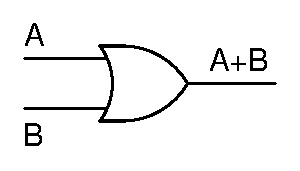
\includegraphics[scale=0.7]{logic/OR.eps}
	\caption{The OR gate outputs A OR B.}
	\label{fig:orgate}
\end{figure} 

\begin{table}[!ht]
	\centering
	\begin{tabular}{| c | c | c |}
		\hline
		A & B & X \\ 
		\hline
		0 & 0 & 0 \\ \hline
		0 & 1 & 1 \\ \hline
		1 & 0 & 1 \\ \hline
		1 & 1 & 1 \\ \hline
	\end{tabular}
	\caption{This is the truth table for an OR gate.}
	\label{table:orgate}
\end{table}

\begin{figure}[!htb]
	\centering
	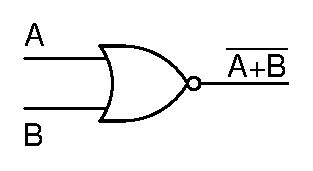
\includegraphics[scale=0.7]{logic/NOR.eps}
	\caption{The NOR gate outputs NOT(A OR B).}
	\label{fig:norgate}
\end{figure} 

\begin{table}[!ht]
	\centering
	\begin{tabular}{| c | c | c |}
		\hline
		A & B & X \\ 
		\hline
		0 & 0 & 1 \\ \hline
		0 & 1 & 0 \\ \hline
		1 & 0 & 0 \\ \hline
		1 & 1 & 0 \\ \hline
	\end{tabular}
	\caption{This is the truth table for an NOR gate.}
	\label{table:norgate}
\end{table}
